\section{GENERAL GEOLOGY (1st floor)}
\label{sec:general-geology}

\subsection{Geological Evolution Through Time}
\label{subsec:geological-evolution}

The Earth has experienced a vast and dynamic history of about 4 billion years. This journey is divided into major geological eons and eras, each defined by important events such as the formation of the crust, shifts in the atmosphere, the rise of life, and tectonic movements. These processes become clearer when explored alongside physical specimens and visual displays, such as those presented at the Ho Chi Minh City Geological Museum.

\textbf{Precambrian Time (Hadean - Archean - Proterozoic; ~4.6 billion - 541 million years ago)}

The Archean Eon (4.0–2.6 billion years ago) represents one of the earliest chapters in Earth's history, when the crust stabilized, continents and oceans first formed, and simple life such as stromatolite-building cyanobacteria appeared, slowly altering the planet's atmosphere. In Vietnam, Archean rocks are found in the Kon Tum geoblock, mainly within the Kan Nack Group. These 3,000-meter-thick metamorphic rocks show complex changes, from granulite facies to amphibolite and greenschist facies, revealing the intense geological processes that shaped the ancient Earth.

\begin{figure}[H]
  \centering
  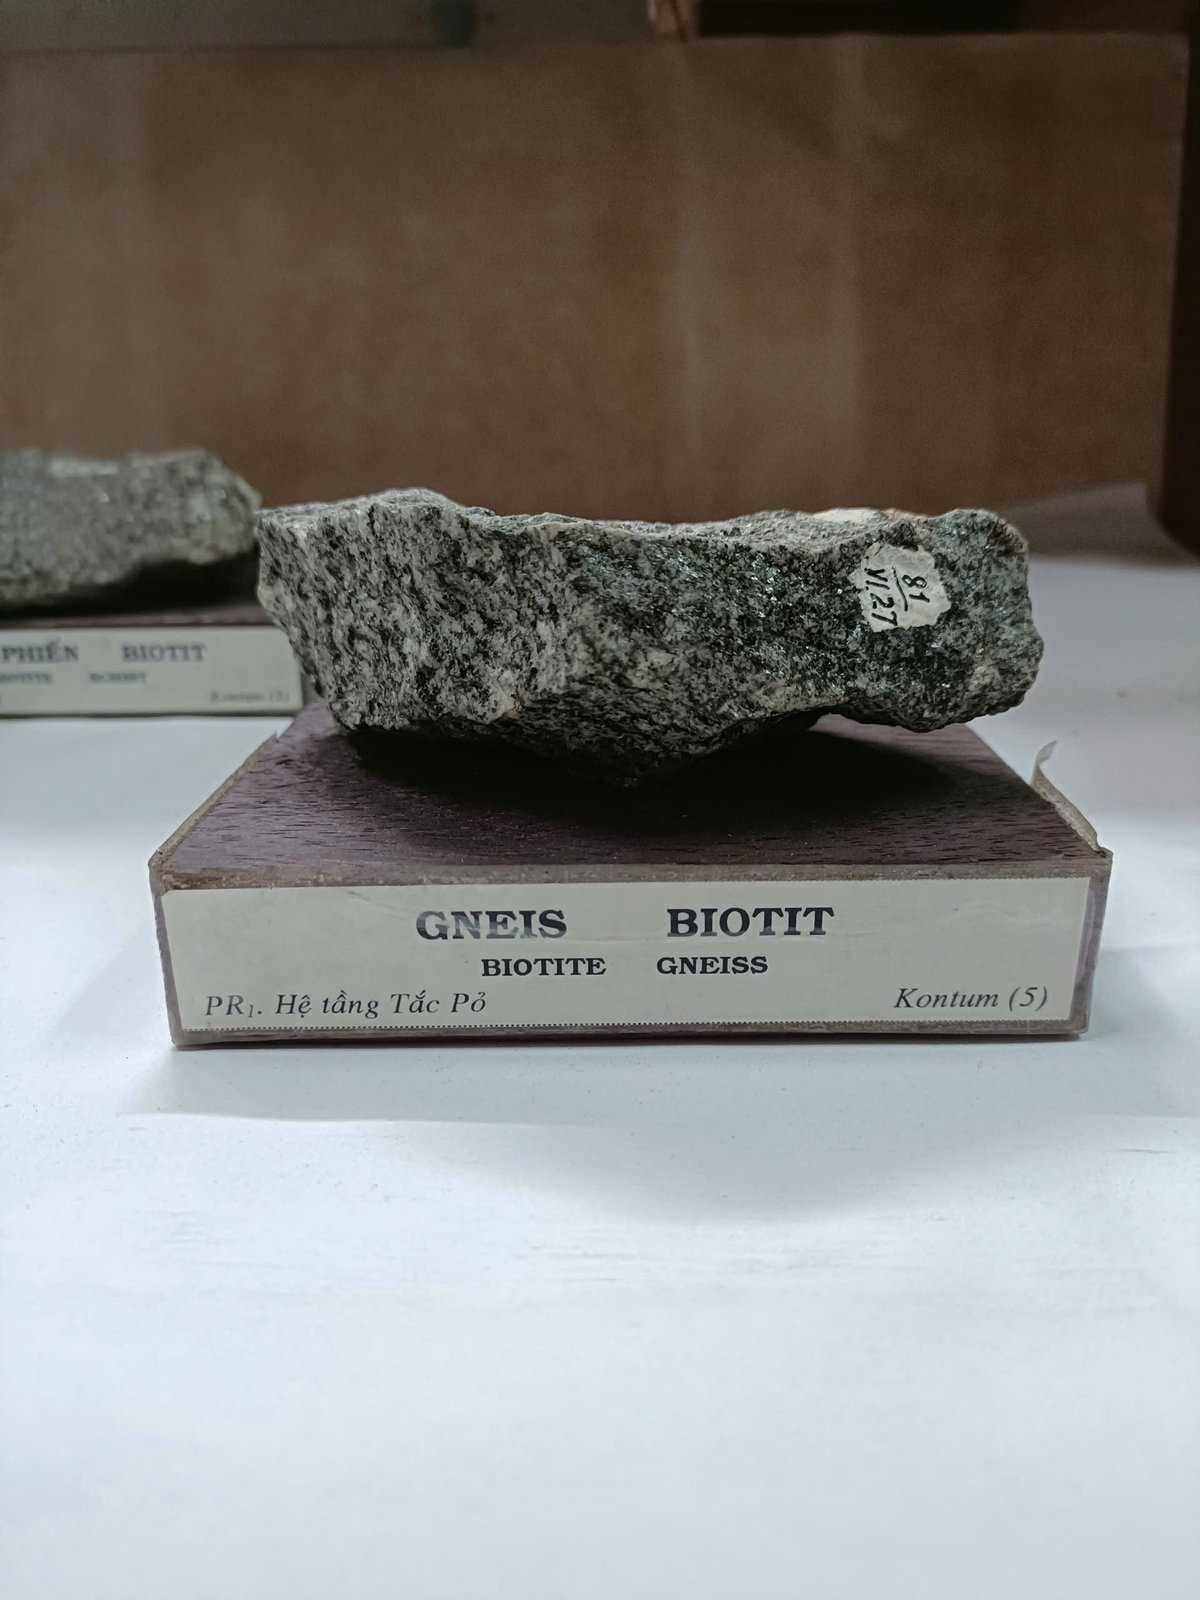
\includegraphics[max width=0.8\linewidth]{graphics/figure_02.jpg}
  \caption{Sample of rock in Archean Eon}
  \label{fig:archean-rock}
\end{figure}

The Proterozoic Eon (2.6 billion to 541 million years ago) saw the Great Oxidation Event, global ice ages called "Snowball Earth," and the rise of the first multicellular life, including the Ediacaran biota. These changes prepared the planet for the Cambrian explosion of life. In Vietnam, rocks from the Proterozoic are found in areas like Red River, Fansipan, Chay River, Ma River, Phu Hoat, and Kon Tum. These include crystalline and metamorphic rocks as well as younger layers that lead into the Cambrian period. Some of these rocks contain fossils of tiny early life forms.

\begin{figure}[H]
  \centering
  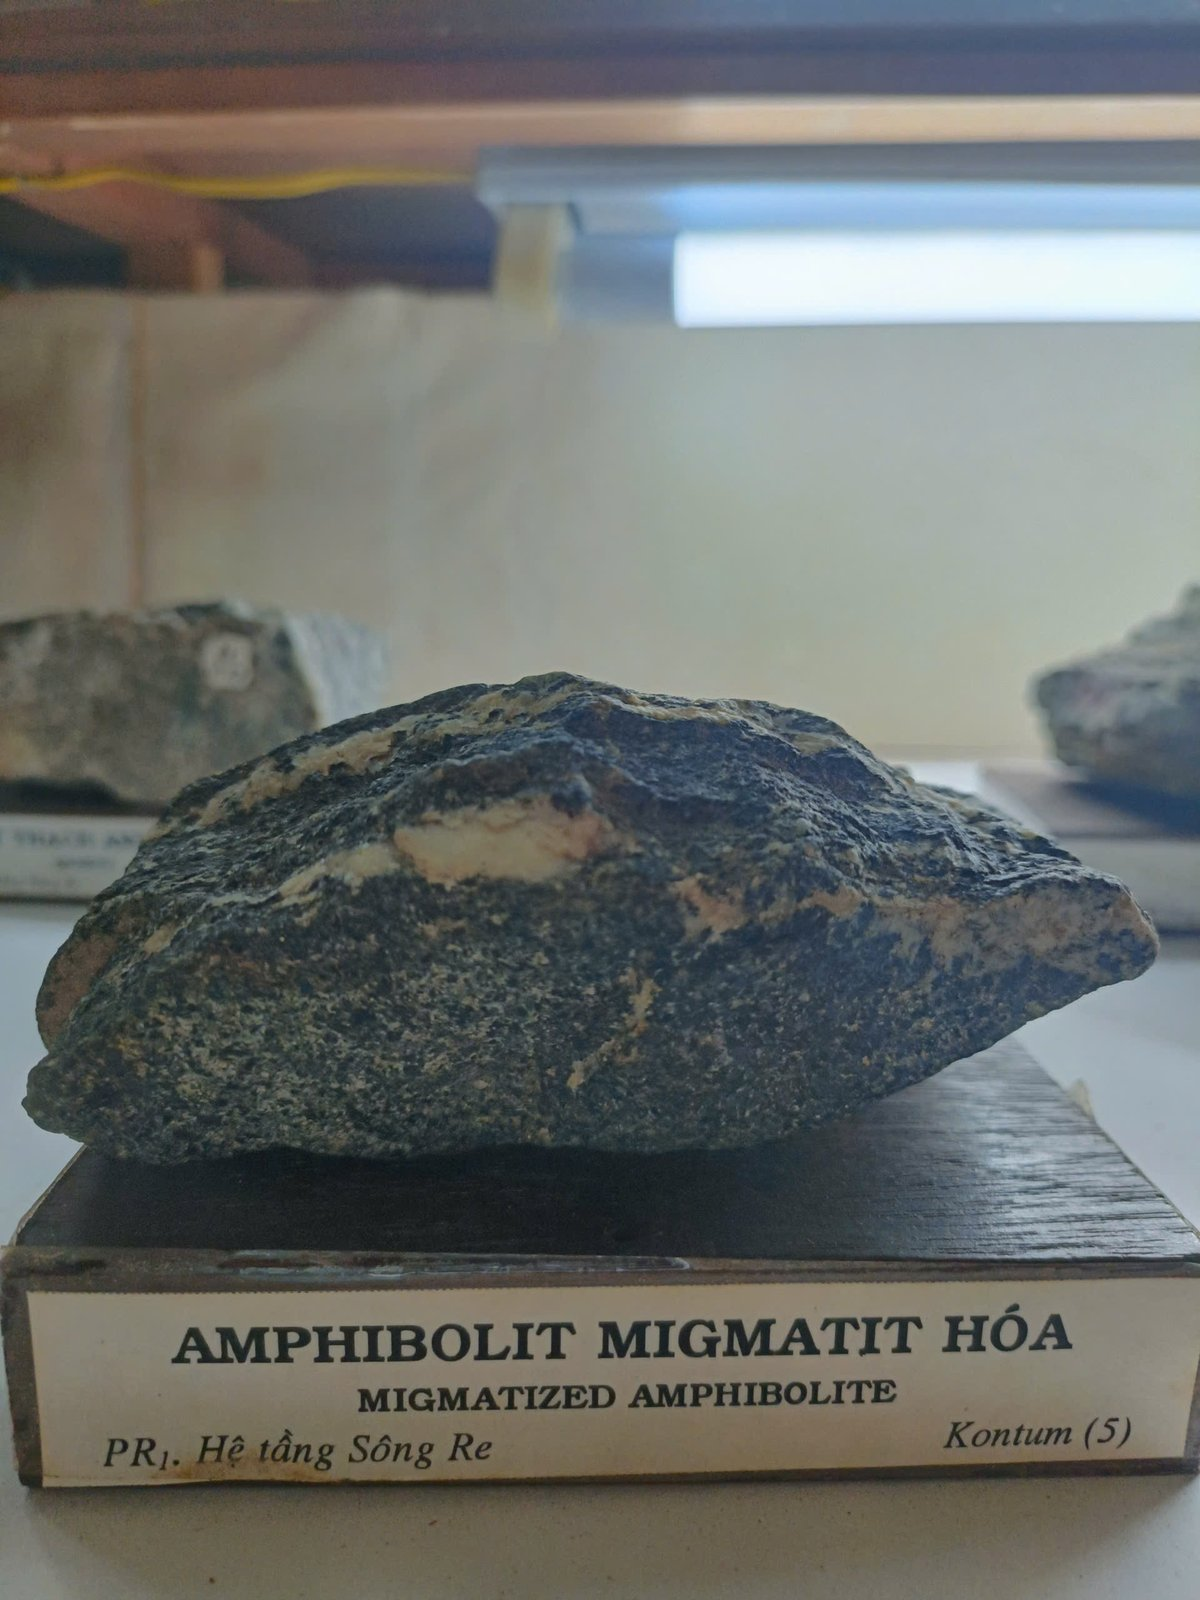
\includegraphics[max width=0.8\linewidth]{graphics/figure_03.jpg}
  \caption{Sample of rock in Proterozoic Eon}
  \label{fig:proterozoic-rock}
\end{figure}

\textbf{Paleozoic Era (541 – 252 million years ago)}

This era began with the Cambrian Explosion, a massive diversification of marine life. It is divided into six periods: Cambrian, Ordovician, Silurian, Devonian, Carboniferous, and Permian. During this time, ocean life expanded rapidly with animals like trilobites, corals, crinoids, brachiopods, graptolites, and cephalopods. Later, plants and amphibians colonized land. The era ended with the Permian-Triassic extinction, the largest known mass extinction, wiping out over 90\% of marine species.

In Vietnam, marine sedimentary rocks with abundant fossils (e.g., corals, brachiopods, trilobites) are found in Northeast Vietnam, such as in Cao Bang and Ha Long Bay. The Truong Son (Annamite) Range began forming due to Caledonian and Hercynian orogenies. Many rocks from the Paleozoic Era can still be found today in regions like North Vietnam, Northwest Vietnam, Northeast Vietnam, and Central Vietnam, where the rocks are made of limestone and other sediments that contain fossils of trilobites, brachiopods, and corals.

At the museum, fossils of corals, mollusks, and petrified wood from areas like Truong Sa (Spratly Islands) and northern Vietnam are exhibited. Geological maps display Paleozoic strata across northern and central Vietnam.

\begin{figure}[H]
  \centering
  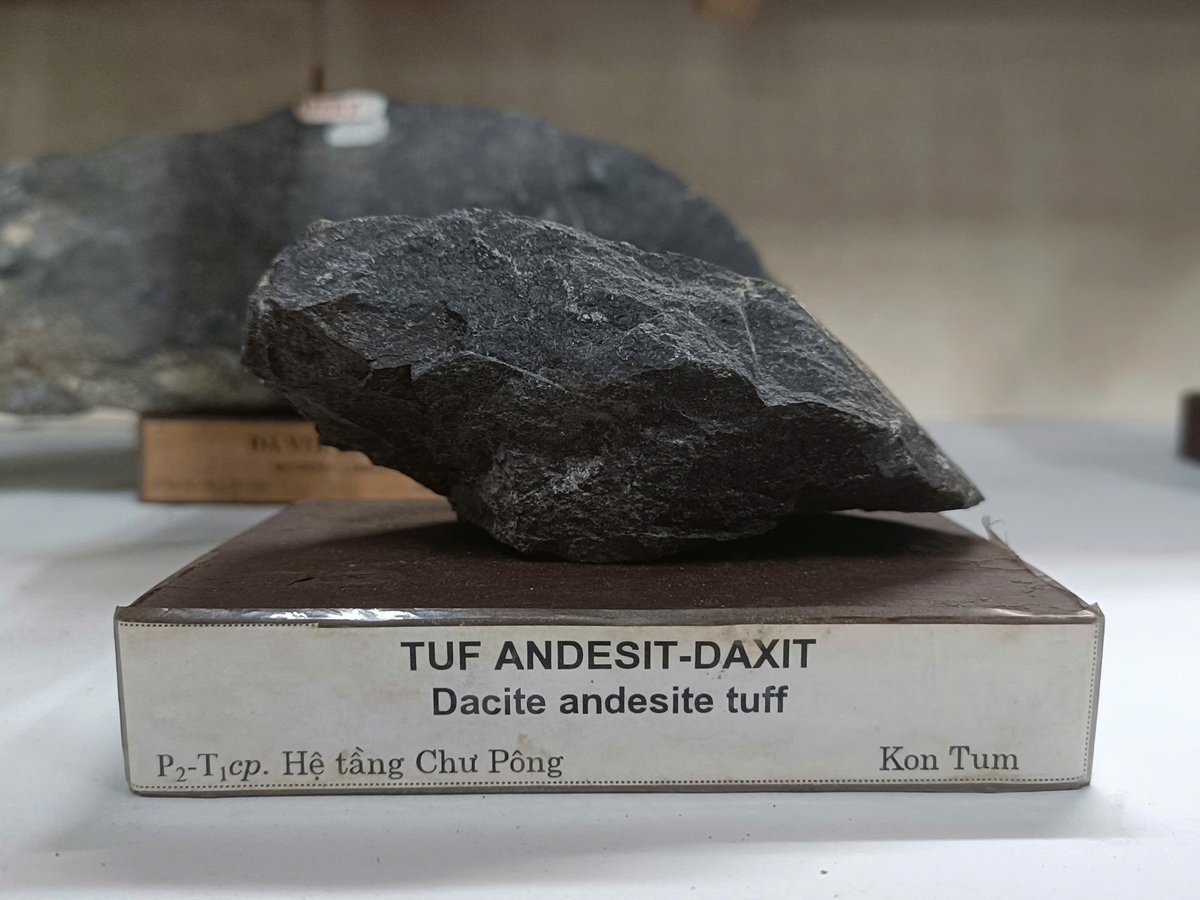
\includegraphics[max width=0.8\linewidth]{graphics/figure_04.jpg}
  \caption{Sample of rock in Paleozoic Era}
  \label{fig:paleozoic-rock}
\end{figure}

\textbf{Mesozoic Era (252 – 66 million years ago)}

Known as the "Age of Dinosaurs," the Mesozoic saw the rise of reptiles, the breakup of Pangaea, and generally warm climates. It is divided into three periods: Triassic, Jurassic, and Cretaceous. This era is famous as the "Age of Reptiles," when dinosaurs, ammonites, and many other creatures lived, along with early plants and marine animals like bivalves and brachiopods. The era ended with the Cretaceous–Paleogene (K–Pg) extinction caused by the Chicxulub impact and Deccan volcanism.

In Vietnam, the Indosinian Orogeny uplifted the Truong Son Range and created sedimentary basins. Volcanic and sedimentary activity occurred in areas like Kon Tum, Son La, and Thanh Hoa. Fossil evidence of dinosaurs and ancient flora has been found in some localities. Mesozoic rocks are found in places such as An Chau, Da River, Hien River, and Southwest. Triassic rocks here contain fossils of ammonites, gastropods, plants, and bivalves. Later, during the Jurassic and Cretaceous, red continental rocks and coal-bearing formations appeared, especially in the North, while volcanic rocks developed in areas like Tam Lang and Tu Le. These layers preserve fossils that show how both land and sea environments changed during this era.

At the museum, basalt and volcanic sediment from this era are displayed in the "Magmatism" section. Fossils and stratigraphic profiles reflect the Mesozoic biosphere and tectonic events.

\begin{figure}[H]
  \centering
  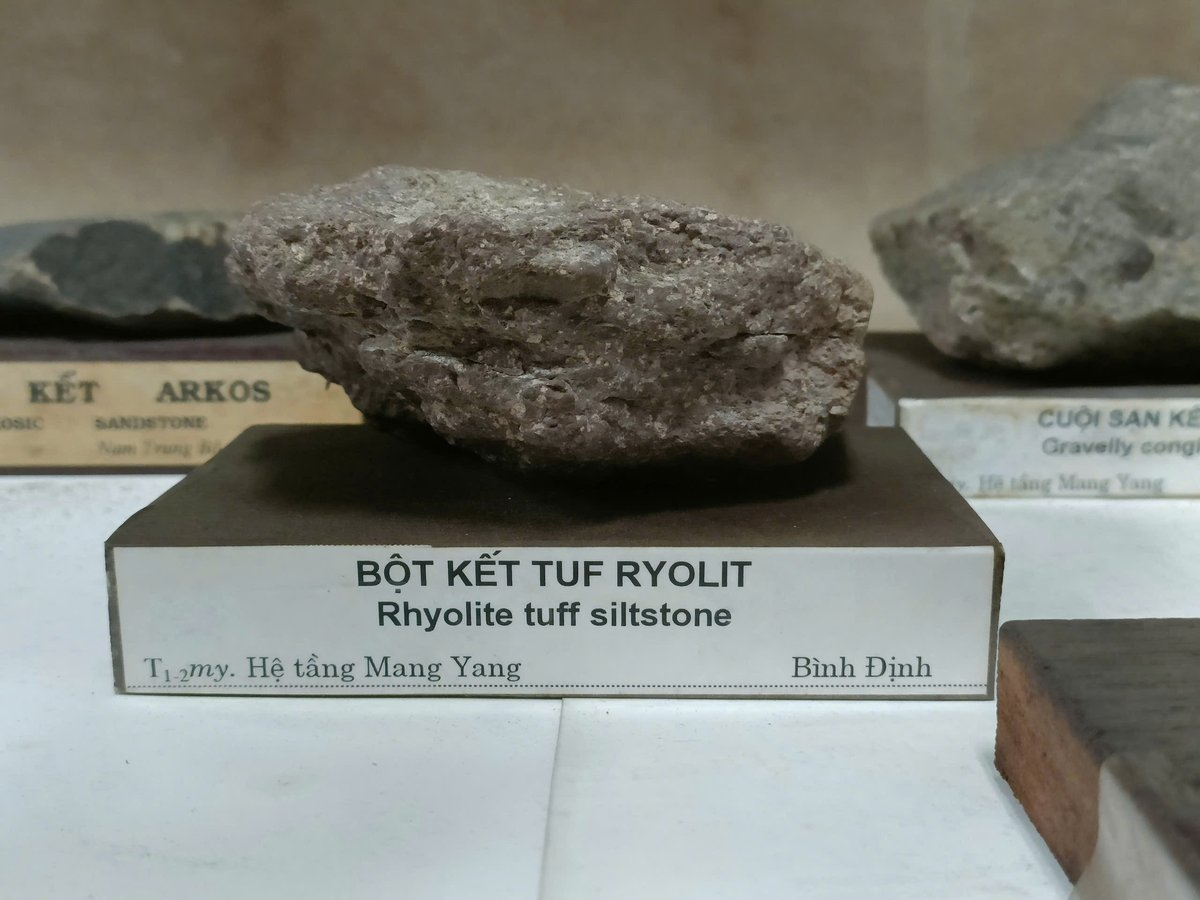
\includegraphics[max width=0.8\linewidth]{graphics/figure_05.jpg}
  \caption{Sample of rock in Mesozoic Era}
  \label{fig:mesozoic-rock}
\end{figure}

\textbf{Cenozoic Era (66 million years ago to present)}

This era features the evolution and dominance of mammals, birds, and eventually humans. Tectonic faulting, glaciations, and sedimentation shaped modern landforms and ecosystems. It is divided into three periods: Paleogene (66–23 million years ago), Neogene (23–2.6 million years ago), and the Quaternary (2.6 million years ago to today). This era is marked by great diversification of life, with many plants, mollusks, diatoms, ostracods, foraminifers, and vertebrates flourishing.

In Vietnam, major faults like the Red River and Song Ca faults influenced the formation of the Cuu Long (Mekong) and Red River basins, rich in oil and gas. The Quaternary Period (~2.58 Ma - present) witnessed alternating glaciations and interglacials, forming the Mekong and Red River deltas through alluvial deposition. Cenozoic rocks are found in regions such as Northwest (Pu Tra, Nam Bay), South Central Coast, and coastal basins. Paleogene rocks are rare, but Neogene sediments are widespread, often containing coal, kaolin, bentonite, and diatomite. These layers also include volcanic rocks, lagoon and delta deposits, and shallow marine formations, preserving fossils that show the rich environments of Vietnam during this era.

At the museum, core samples of crude oil from the Cuu Long basin (collected in the 1980s) are on display. Sediment cores and alluvial rock samples reflect recent geological processes, showcased in the "Fuel Group" and sedimentary sections.

\begin{figure}[H]
  \centering
  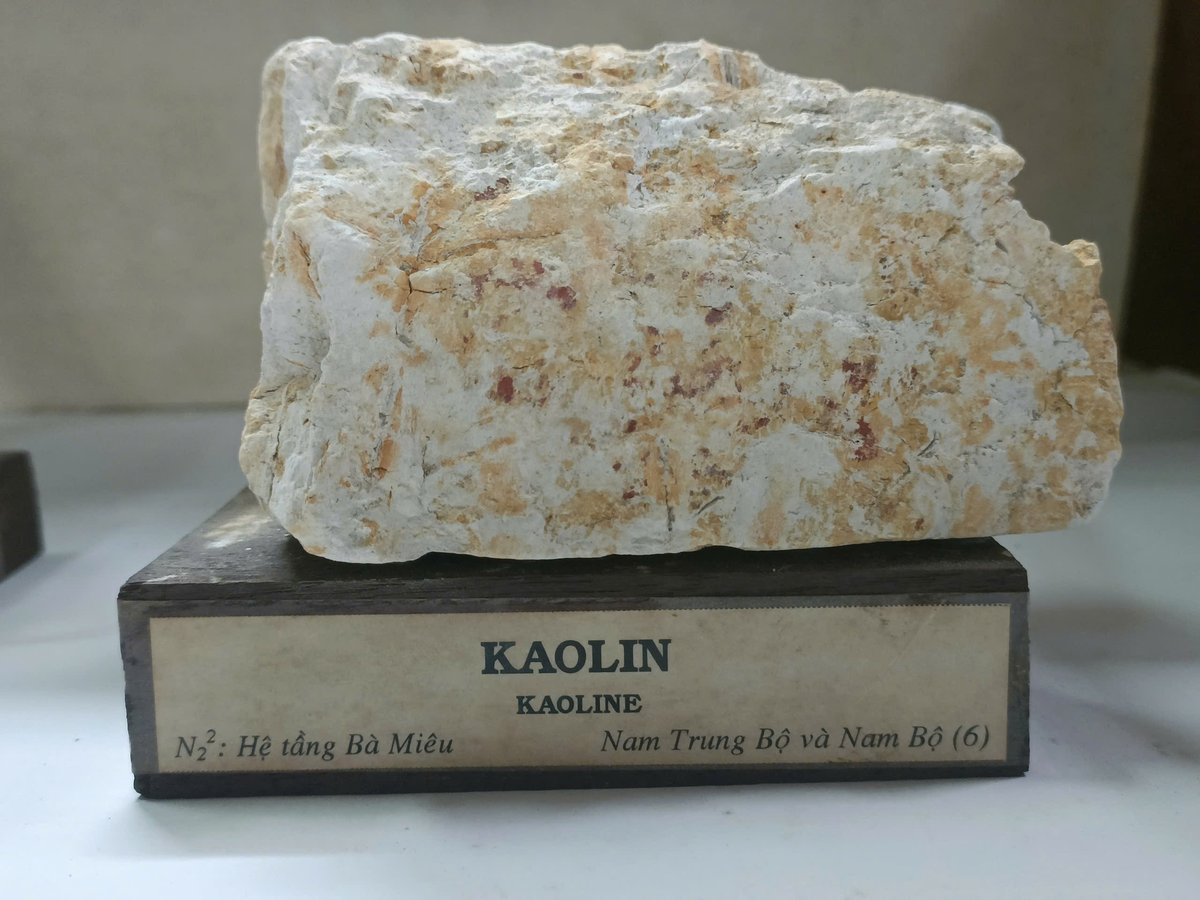
\includegraphics[max width=0.8\linewidth]{graphics/figure_06.jpg}
  \caption{Sample of rock in Cenozoic Era}
  \label{fig:cenozoic-rock}
\end{figure}

\subsection{Geological Processes}
\label{subsec:geological-processes}

Geological processes are natural forces that continuously shape and alter both the Earth's surface and its interior. At the Ho Chi Minh City Geological Museum, visitors were introduced to six key geological processes through rock samples, models, and diagrams. These processes—ranging from extraterrestrial impacts to deep-earth activity and surface transformations—drive the creation, modification, and recycling of Earth's materials. The museum's exhibits illustrated how each process contributes to the formation of various rocks and landforms, highlighting the dynamic and interconnected system of the geological cycle.

\textbf{Cosmic Process}

Although no meteorite samples were displayed during the visit, the cosmic process remains essential in Earth's geological history. It refers to extraterrestrial impacts, especially meteorites, which helped shape the early Earth. These collisions formed craters, altered surface rocks, and delivered elements like iron, nickel, and platinum - key components of Earth's crust and core. Despite the lack of exhibits, this process highlights the planet's cosmic origins and is widely studied through global meteorite discoveries.

\textbf{Tectonic Process}

Tectonic processes involve the movement of the Earth's lithospheric plates. These dynamic movements are responsible for geological phenomena such as earthquakes, volcanic eruptions, mountain formation, and continental drift.

At the museum, this process was illustrated through global tectonic maps and a three-dimensional model of plate boundaries, showing the locations and interactions between major tectonic plates around the world. These materials effectively demonstrate how plates move and interact through different boundary types:

\begin{itemize}
  \item Divergent boundaries, where plates move apart and new crust forms;
  \item Convergent boundaries, where plates collide, leading to subduction and mountain building;
  \item Transform boundaries, where plates slide past each other, often causing earthquakes.
\end{itemize}

The exhibit helps explain how these boundary interactions drive geological activity and continuously shape the Earth's surface.

\textbf{Magmatic Process}

Magmatic processes are responsible for the formation of igneous rocks through the cooling and solidification of magma. These rocks differ in texture and composition depending on where and how quickly the magma cools.

In the museum exhibit, igneous rocks were organized into two main groups. Extrusive rocks, such as basalt and andesite, are formed from lava that cools quickly at the surface. Because the cooling is rapid, crystals don't have time to grow large, resulting in a fine-grained texture. Intrusive rocks, like granite and diorite, form deep underground where magma cools slowly over extended periods. This slow cooling allows large crystals to develop, giving the rocks a coarse, crystalline texture.

The museum displays showed how different cooling environments produce rocks with distinct characteristics, helping visitors understand the relationship between geological processes and rock formation.

\begin{figure}[H]
  \centering
  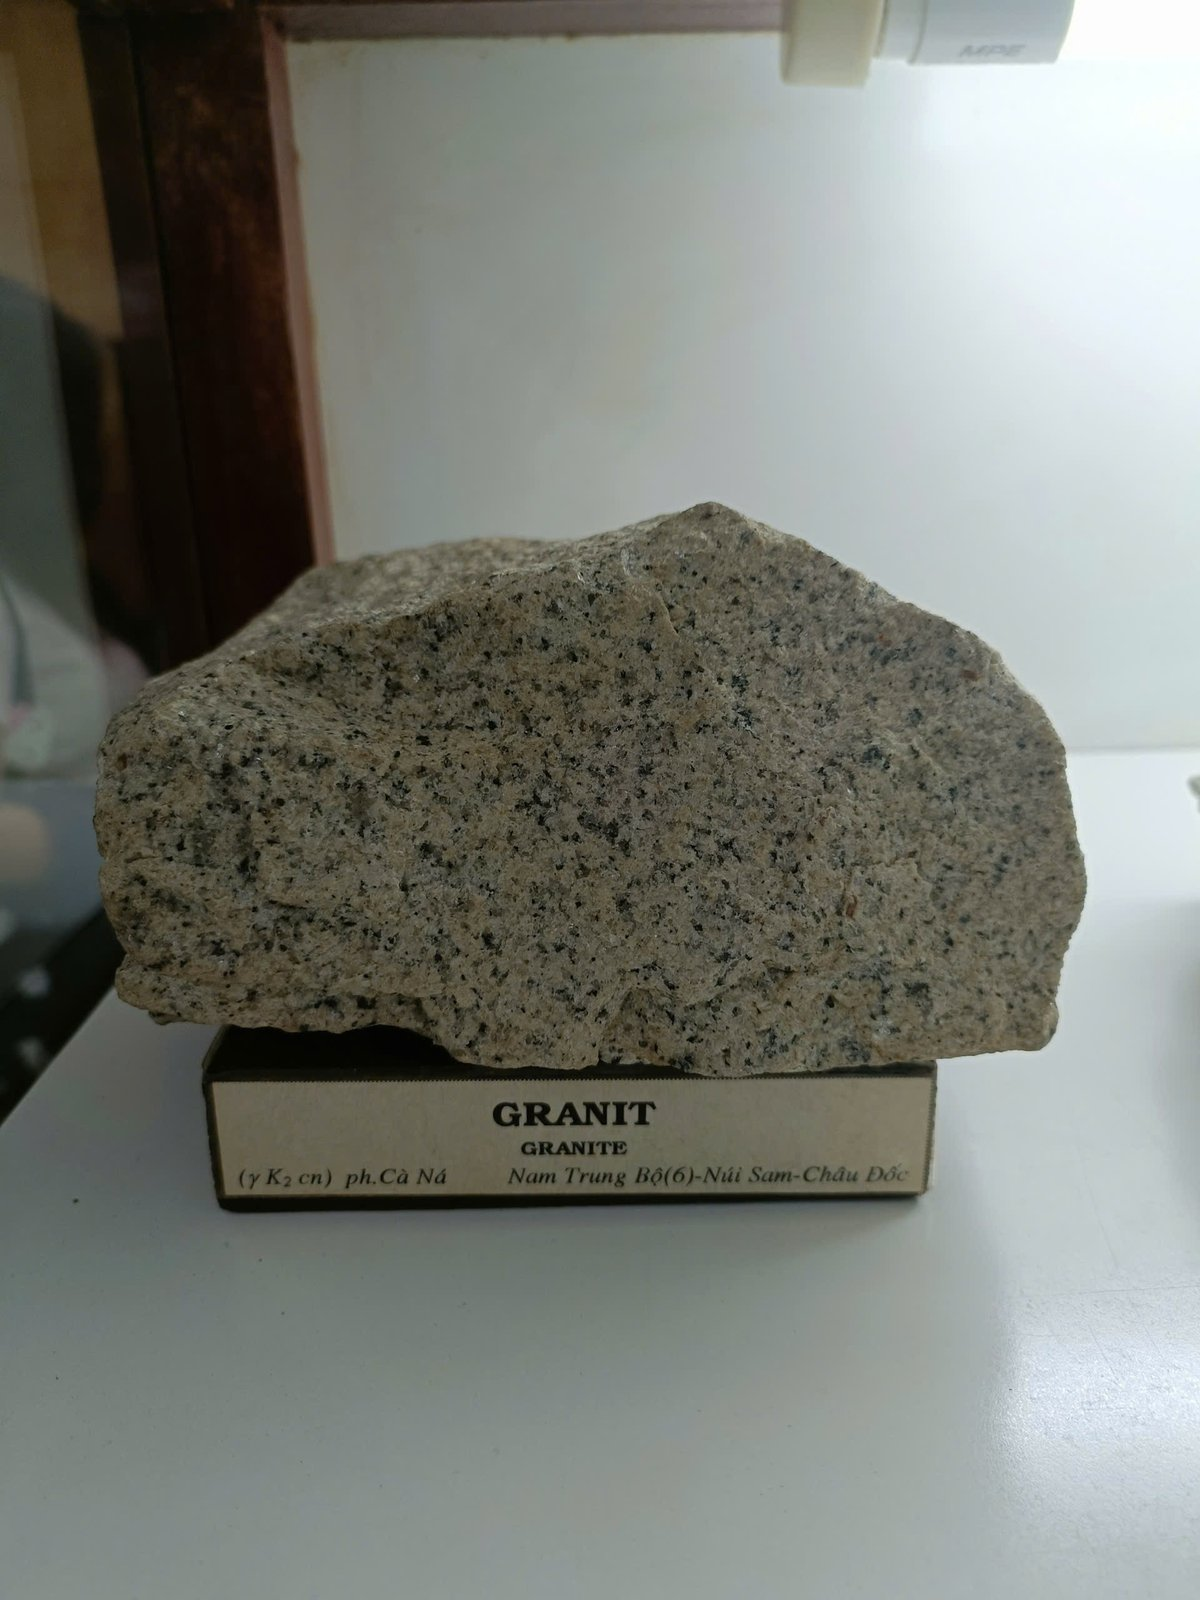
\includegraphics[max width=0.8\linewidth]{graphics/figure_07.jpg}
  \caption{Sample of intrusive igneous rock}
  \label{fig:intrusive-igneous}
\end{figure}

\textbf{Metamorphic Process}

Metamorphism happens when existing rocks undergo high heat, strong pressure, or interaction with reactive fluids, leading them to change into new rock types. At the museum, specimens like schist, gneiss, slate, quartzite, and marble were displayed, each representing different metamorphic environments.

One highlighted example was marble, which develops from limestone through contact metamorphism. The exhibit also included diagrams of metamorphic facies and processes, illustrating how different conditions drive these rock transformations.

\begin{figure}[H]
  \centering
  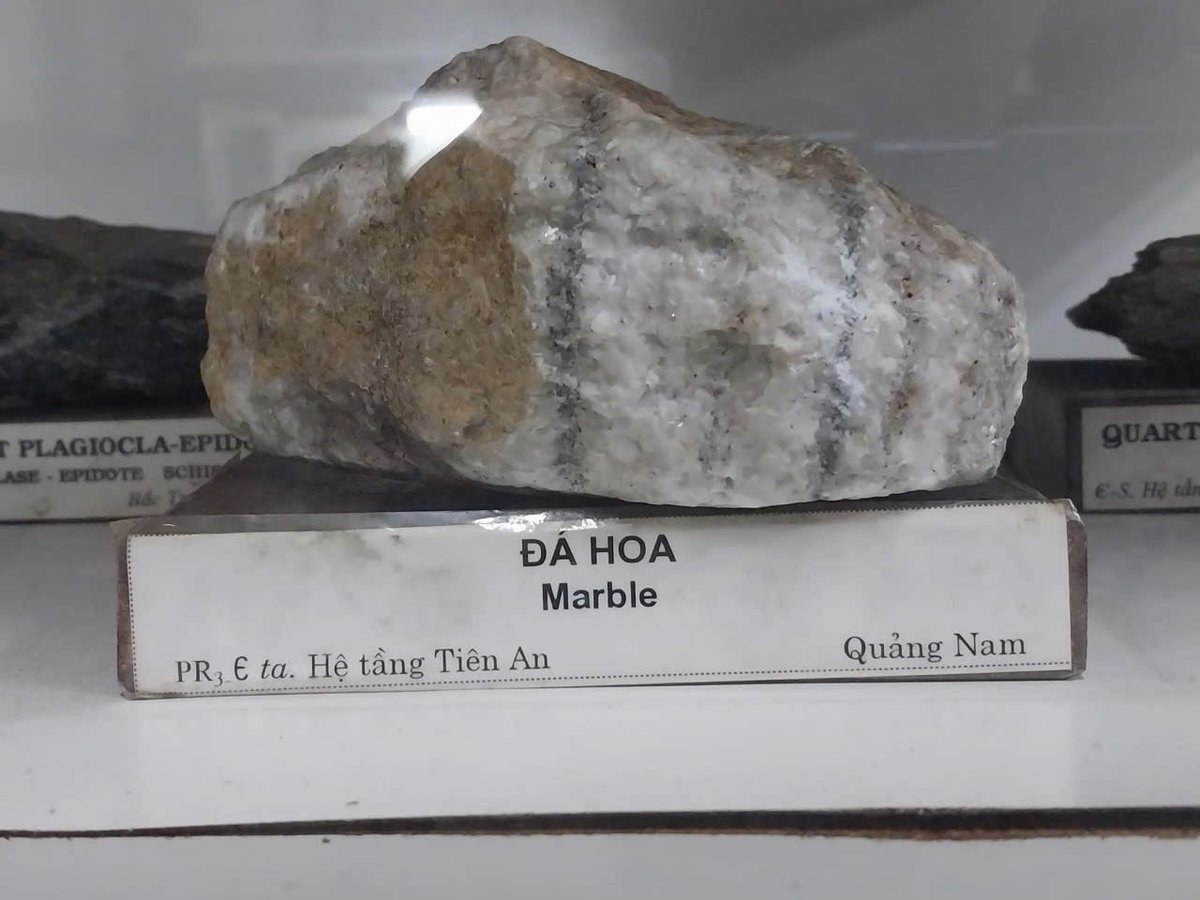
\includegraphics[max width=0.8\linewidth]{graphics/figure_08.jpg}
  \caption{Sample of Marble}
  \label{fig:marble}
\end{figure}

\textbf{Sedimentary Process}

Sedimentary processes occur when materials from older rocks or biological sources are gathered, compressed, and cemented together, resulting in sedimentary rocks that typically show layered structures.

\begin{itemize}
  \item Mechanical sedimentation produces rocks such as sandstone and conglomerate, created from the physical breakdown and accumulation of rock fragments.
  \item Chemical sedimentation is seen in rocks like limestone, which forms when minerals precipitate from water-rich solutions.
\end{itemize}

\begin{figure}[H]
  \centering
  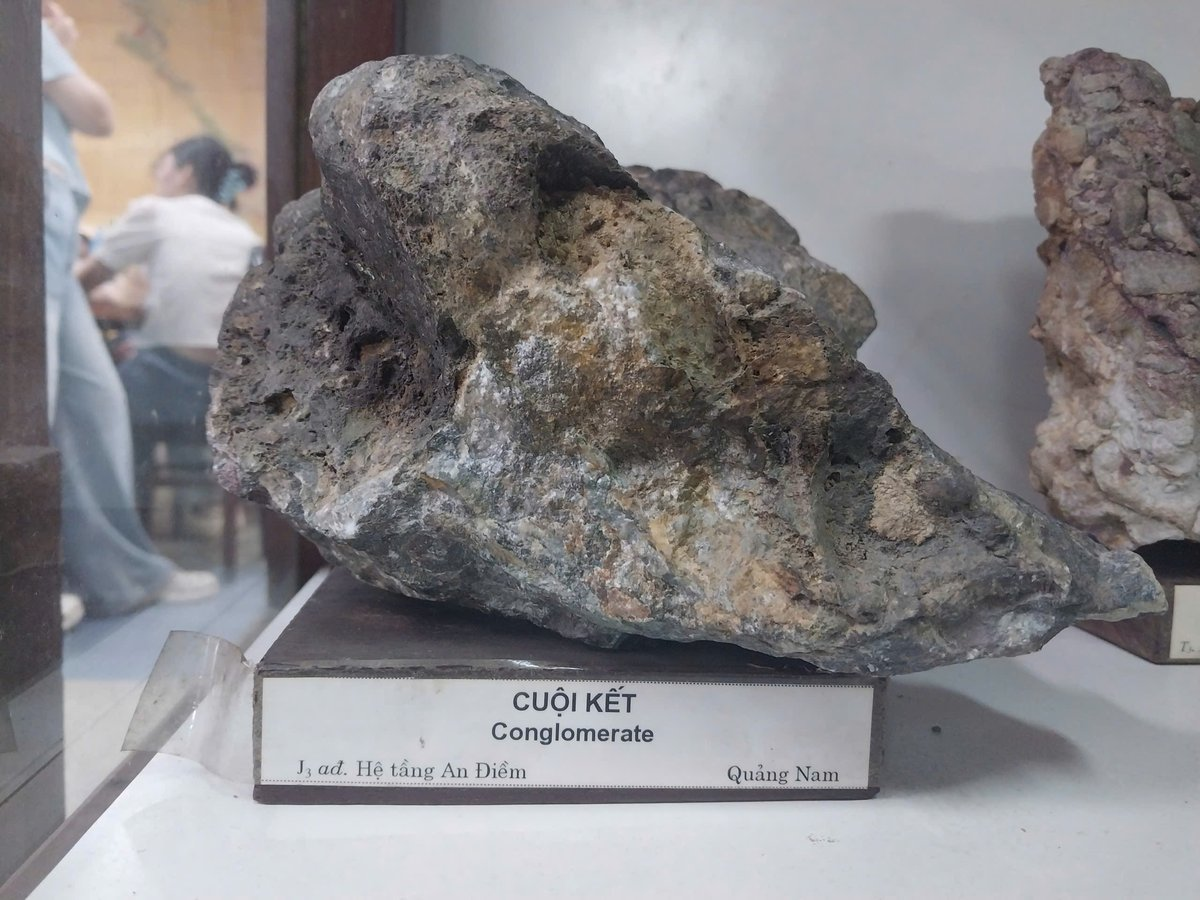
\includegraphics[max width=0.8\linewidth]{graphics/figure_09.jpg}
  \caption{Sample of Mechanical sedimentation rock}
  \label{fig:mechanical-sedimentation}
\end{figure}

\textbf{Weathering Process}

Weathering is the natural process that breaks down rocks at Earth's surface through the effects of wind, rainfall, temperature changes, and chemical reactions. At the museum, this was demonstrated with diagrams and rock samples that showed how rocks are altered by different types of weathering.

Examples included mechanical weathering, such as rock fragmentation and exfoliation, and chemical weathering, like the oxidation of iron on rock surfaces. These displays highlighted weathering's important role in the rock cycle, as it produces loose sediments that can later compact and cement to form sedimentary rocks.

\begin{figure}[H]
  \centering
  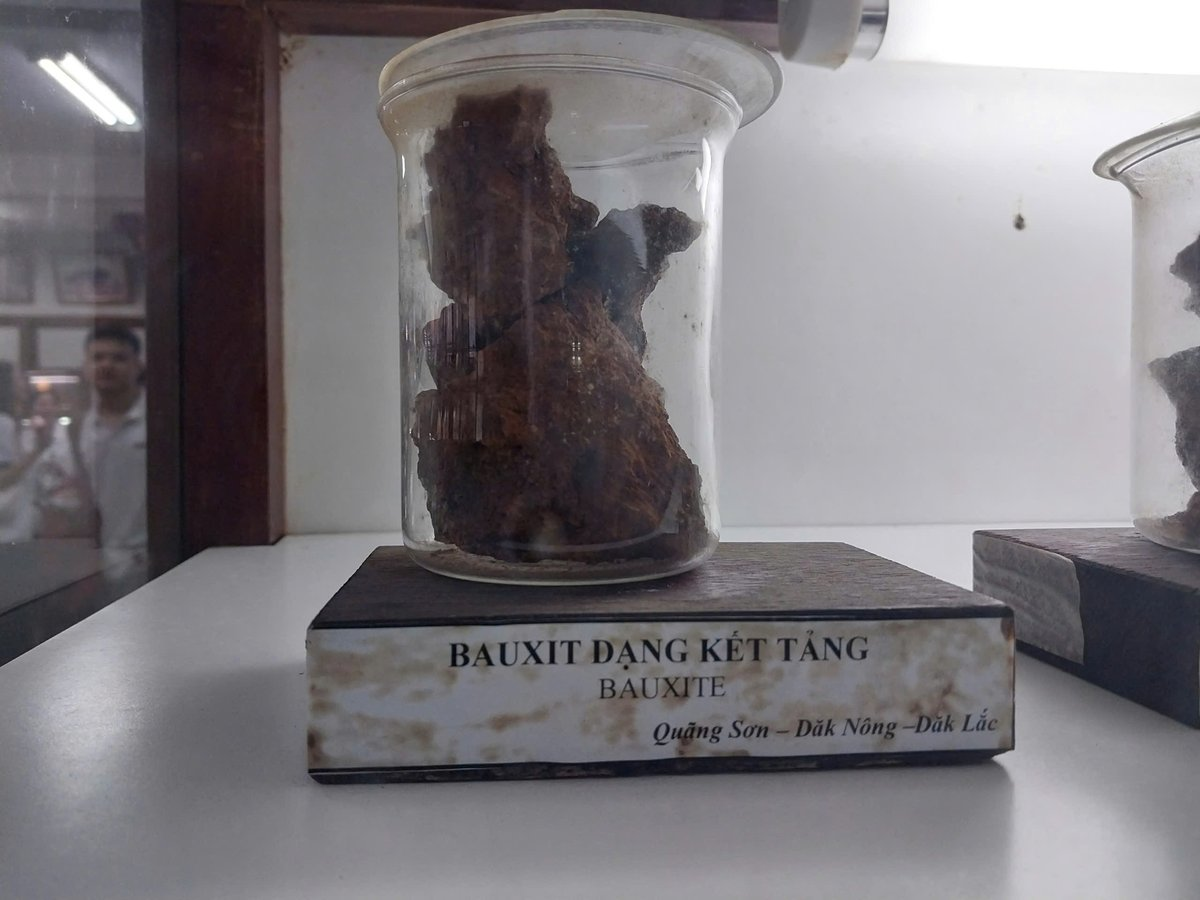
\includegraphics[max width=0.8\linewidth]{graphics/figure_10.jpg}
\caption{Sample of Bauxite}
\label{fig:bauxite}
\end{figure}